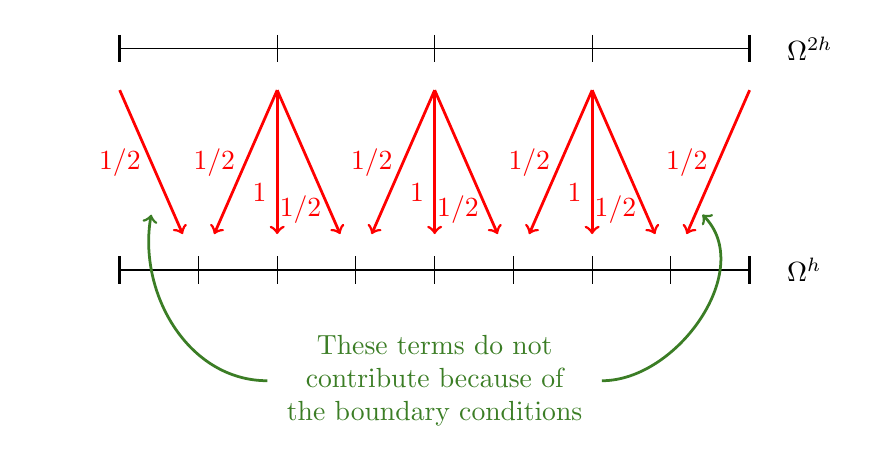
\begin{tikzpicture}
    \draw (0, -8em) node[right]{\phantom{$\quad \Omega^{h}$}}-- (8, -8em) node[right]{$\quad \Omega^{h}$};
    \draw[line width = 1pt] (0, .5em) -- (0, -.5em) node[below] {} ;
    \draw[line width = 1pt] (8, .5em) -- (8, -.5em) node[below] {} ;
    \foreach \x in {2, 4, 6}
        \draw[shift={(\x, 0)}] (0, .5em) -- (0, -.5em);

    \draw (0, 0) node[left]{\phantom{$\quad \Omega^{2h}$}} -- (8, 0) node[right]{$\quad \Omega^{2h}$};
    \draw[line width = 1pt] (0, -7.5em) -- (0, -8.5em) node[below] {} ;
    \draw[line width = 1pt] (8, -7.5em) -- (8, -8.5em) node[below] {} ;
    \foreach \x in {1, ..., 7}
        \draw[shift={(\x, 0)}] (0, -7.5em) -- (0, -8.5em);
    
    {
    \color{red}
    %% n = 1
    
    \draw[->, line width=1pt] 
    (0, -1.5em) 
    -- 
    (0.8, -6.7em) node[midway, left]{1/2} ;
    \draw[->, line width=1pt] 
    (2, -1.5em) 
    -- 
    (1.2, -6.7em)node[midway,left]{1/2} 
    ;
    \draw[->, line width=1pt] 
    (2, -1.5em)  
    -- 
    (2, -6.7em) node[left, yshift=1.5em]{1} ;
    \draw[->, line width=1pt] 
    (2, -1.5em)  
    -- 
    (2.8, -6.7em) node[left, yshift=.9em, xshift=-.3em]{1/2} ;
    
    \draw[->, line width=1pt] 
    (4, -1.5em) 
    -- 
    (3.2, -6.7em)node[midway,left]{1/2} 
    ;
    \draw[->, line width=1pt] 
    (4, -1.5em)  
    -- 
    (4, -6.7em) node[left, yshift=1.5em]{1} ;
    \draw[->, line width=1pt] 
    (4, -1.5em)  
    -- 
    (4.8, -6.7em) node[left, yshift=.9em, xshift=-.3em]{1/2} ;
    
    \draw[->, line width=1pt] 
    (6, -1.5em) 
    -- 
    (5.2, -6.7em)node[midway,left]{1/2} 
    ;
    \draw[->, line width=1pt] 
    (6, -1.5em)  
    -- 
    (6, -6.7em) node[left, yshift=1.5em]{1} ;
    \draw[->, line width=1pt] 
    (6, -1.5em)  
    -- 
    (6.8, -6.7em) node[left, yshift=.9em, xshift=-.3em]{1/2} ;
    \draw[->, line width=1pt] 
    (8, -1.5em) 
    -- 
    (7.2, -6.7em)node[midway,left]{1/2} 
    ;
    }
    {
    \color{OliveGreen}
    \node[text width=4cm,align=center] (text) at (4, -12em) {These terms do not contribute because of the boundary conditions};
    \draw[->, line width=1pt] (text.west) to[out=180, in=-100] (0.4, -6em);
    \draw[->, line width=1pt] (text.east) to[out=0, in=-45] (7.4, -6em);
    }
\end{tikzpicture}
